\documentclass[twoside]{book}

% Packages required by doxygen
\usepackage{fixltx2e}
\usepackage{calc}
\usepackage{doxygen}
\usepackage[export]{adjustbox} % also loads graphicx
\usepackage{graphicx}
\usepackage[utf8]{inputenc}
\usepackage{makeidx}
\usepackage{multicol}
\usepackage{multirow}
\PassOptionsToPackage{warn}{textcomp}
\usepackage{textcomp}
\usepackage[nointegrals]{wasysym}
\usepackage[table]{xcolor}

% Font selection
\usepackage[T1]{fontenc}
\usepackage[scaled=.90]{helvet}
\usepackage{courier}
\usepackage{amssymb}
\usepackage{sectsty}
\renewcommand{\familydefault}{\sfdefault}
\allsectionsfont{%
  \fontseries{bc}\selectfont%
  \color{darkgray}%
}
\renewcommand{\DoxyLabelFont}{%
  \fontseries{bc}\selectfont%
  \color{darkgray}%
}
\newcommand{\+}{\discretionary{\mbox{\scriptsize$\hookleftarrow$}}{}{}}

% Page & text layout
\usepackage{geometry}
\geometry{%
  a4paper,%
  top=2.5cm,%
  bottom=2.5cm,%
  left=2.5cm,%
  right=2.5cm%
}
\tolerance=750
\hfuzz=15pt
\hbadness=750
\setlength{\emergencystretch}{15pt}
\setlength{\parindent}{0cm}
\setlength{\parskip}{3ex plus 2ex minus 2ex}
\makeatletter
\renewcommand{\paragraph}{%
  \@startsection{paragraph}{4}{0ex}{-1.0ex}{1.0ex}{%
    \normalfont\normalsize\bfseries\SS@parafont%
  }%
}
\renewcommand{\subparagraph}{%
  \@startsection{subparagraph}{5}{0ex}{-1.0ex}{1.0ex}{%
    \normalfont\normalsize\bfseries\SS@subparafont%
  }%
}
\makeatother

% Headers & footers
\usepackage{fancyhdr}
\pagestyle{fancyplain}
\fancyhead[LE]{\fancyplain{}{\bfseries\thepage}}
\fancyhead[CE]{\fancyplain{}{}}
\fancyhead[RE]{\fancyplain{}{\bfseries\leftmark}}
\fancyhead[LO]{\fancyplain{}{\bfseries\rightmark}}
\fancyhead[CO]{\fancyplain{}{}}
\fancyhead[RO]{\fancyplain{}{\bfseries\thepage}}
\fancyfoot[LE]{\fancyplain{}{}}
\fancyfoot[CE]{\fancyplain{}{}}
\fancyfoot[RE]{\fancyplain{}{\bfseries\scriptsize Generated by Doxygen }}
\fancyfoot[LO]{\fancyplain{}{\bfseries\scriptsize Generated by Doxygen }}
\fancyfoot[CO]{\fancyplain{}{}}
\fancyfoot[RO]{\fancyplain{}{}}
\renewcommand{\footrulewidth}{0.4pt}
\renewcommand{\chaptermark}[1]{%
  \markboth{#1}{}%
}
\renewcommand{\sectionmark}[1]{%
  \markright{\thesection\ #1}%
}

% Indices & bibliography
\usepackage{natbib}
\usepackage[titles]{tocloft}
\setcounter{tocdepth}{3}
\setcounter{secnumdepth}{5}
\makeindex

% Hyperlinks (required, but should be loaded last)
\usepackage{ifpdf}
\ifpdf
  \usepackage[pdftex,pagebackref=true]{hyperref}
\else
  \usepackage[ps2pdf,pagebackref=true]{hyperref}
\fi
\hypersetup{%
  colorlinks=true,%
  linkcolor=blue,%
  citecolor=blue,%
  unicode%
}

% Custom commands
\newcommand{\clearemptydoublepage}{%
  \newpage{\pagestyle{empty}\cleardoublepage}%
}

\usepackage{caption}
\captionsetup{labelsep=space,justification=centering,font={bf},singlelinecheck=off,skip=4pt,position=top}

%===== C O N T E N T S =====

\begin{document}

% Titlepage & ToC
\hypersetup{pageanchor=false,
             bookmarksnumbered=true,
             pdfencoding=unicode
            }
\pagenumbering{alph}
\begin{titlepage}
\vspace*{7cm}
\begin{center}%
{\Large Whatsapp Web A\+PI \\[1ex]\large 1 }\\
\vspace*{1cm}
{\large Generated by Doxygen 1.8.13}\\
\end{center}
\end{titlepage}
\clearemptydoublepage
\pagenumbering{roman}
\tableofcontents
\clearemptydoublepage
\pagenumbering{arabic}
\hypersetup{pageanchor=true}

%--- Begin generated contents ---
\chapter{Whatsapp api}
\label{index}\hypertarget{index}{}\hypertarget{index_intro_sec}{}\section{Introduction}\label{index_intro_sec}
This is an api made for automating Whatsapp behaviour

possible uses for this A\+PI\+:
\begin{DoxyItemize}
\item Service of sorts
\item Personal usage
\item Others...
\end{DoxyItemize}\hypertarget{index_terms_sec}{}\section{Terms of Use}\label{index_terms_sec}

\begin{DoxyItemize}
\item You will N\+OT use this A\+PI for marketing purposes (spam, massive sending...).
\item We do N\+OT give support to anyone that wants this A\+PI to send massive messages or similar.
\item We reserve the right to block any user of this repository that does not meet these conditions.
\item We are not associated with Whatsapp(tm) or Facebook(tm)
\end{DoxyItemize}\hypertarget{index_install_sec}{}\section{Installation}\label{index_install_sec}
\hypertarget{index_step1}{}\subsection{Step 1\+: Cloning the repository}\label{index_step1}
This can be done by simply going to https\+://github.com/\+Iwra\+Studios/\+Whatsapp-\/\+Bot and clicking clone or download and downloading the zip file

On linux machines it can be easier to do (although you won\textquotesingle{}t have VS so how does that work?) ~\newline
 git clone \href{mailto:git@github.com}{\tt git@github.\+com}\+:Iwra\+Studios/\+Whatsapp-\/\+Bot.\+git ~\newline
 or ~\newline
 git clone github.\+com/\+Iwra\+Studios/\+Whatsapp-\/\+Bot.git ~\newline
 \hypertarget{index_step2}{}\subsection{Step 2\+: Intergrating it into your own project}\label{index_step2}
\subsubsection*{Method 1\+:}

Assuming you already have an VS C\# project just right click on\+: Solution \char`\"{}your\+\_\+project\char`\"{}, in Solution Explorer ~\newline
 going to \char`\"{}\+Add $>$\char`\"{} and choosing existing project, then navigate to Whatsapp-\/\+Bot-\/master\textbackslash{}\hyperlink{namespace_web_whatsapp_a_p_i}{Web\+Whatsapp\+A\+PI}\textbackslash{}Web\+Whatsapp\+A\+P\+I.\+csproj ~\newline
 and clicking \char`\"{}\+Open\char`\"{} ~\newline
 Now you can add it as a refrence by right-\/clicking Refrences in your project, going to Projects and checking the checkmark ~\newline
 Aaaand your done. ~\newline
 \subsubsection*{Method 2\+:}

As an alternative method you can open the project Whatsapp\+Bot.\+sln or Web\+Whatsapp\+A\+P\+I.\+csproj and building it ~\newline
 Then you can copy the .dll\textquotesingle{}s and .exe\textquotesingle{}s from Web\+Whatsapp\+A\+PI\textbackslash{}$\ast$\textbackslash{}bin\textbackslash{}$\ast$.dll and Web\+Whatsapp\+A\+P\+I$\ast$\textbackslash{}bin\textbackslash{}$\ast$.exe ~\newline
 after you have done all that you can add the dll\textquotesingle{}s as a refrence by going to refrences (right-\/click), clicking browse and going to the dll\textquotesingle{}s ~\newline
 when building your project you will have to either\+: ~\newline
 copy the exe\textquotesingle{}s to the \%$\ast$\textbackslash{}bin\textbackslash{} directory of your project ~\newline
 or ~\newline
 Adding a build step that does this for you ~\newline
 \hypertarget{index_step3}{}\subsection{Step 3\+: Using it}\label{index_step3}
I could write an whole article about how to use the api but that is why these docs exist ~\newline
 If you don\textquotesingle{}t know how to do something look at the examples or the api docs ~\newline
 If you, after you did that, still don\textquotesingle{}t know how to do something go to https\+://github.com/\+Iwra\+Studios/\+Whatsapp-\/\+Bot/issues and create a new issue ~\newline

\chapter{Namespace Index}
\section{Namespace List}
Here is a list of all documented namespaces with brief descriptions\+:\begin{DoxyCompactList}
\item\contentsline{section}{\hyperlink{namespace_firefox_example}{Firefox\+Example} }{\pageref{namespace_firefox_example}}{}
\item\contentsline{section}{\hyperlink{namespace_web_whatsapp_a_p_i}{Web\+Whatsapp\+A\+PI} }{\pageref{namespace_web_whatsapp_a_p_i}}{}
\item\contentsline{section}{\hyperlink{namespace_web_whatsapp_a_p_i_1_1_chrome}{Web\+Whatsapp\+A\+P\+I.\+Chrome} }{\pageref{namespace_web_whatsapp_a_p_i_1_1_chrome}}{}
\item\contentsline{section}{\hyperlink{namespace_web_whatsapp_a_p_i_1_1_firefox}{Web\+Whatsapp\+A\+P\+I.\+Firefox} }{\pageref{namespace_web_whatsapp_a_p_i_1_1_firefox}}{}
\end{DoxyCompactList}

\chapter{Hierarchical Index}
\section{Class Hierarchy}
This inheritance list is sorted roughly, but not completely, alphabetically\+:\begin{DoxyCompactList}
\item \contentsline{section}{Web\+Whatsapp\+A\+P\+I.\+Base\+Class.\+Auto\+Save\+Settings}{\pageref{class_web_whatsapp_a_p_i_1_1_base_class_1_1_auto_save_settings}}{}
\item \contentsline{section}{Web\+Whatsapp\+A\+P\+I.\+Base\+Class}{\pageref{class_web_whatsapp_a_p_i_1_1_base_class}}{}
\begin{DoxyCompactList}
\item \contentsline{section}{Web\+Whatsapp\+A\+P\+I.\+Firefox.\+Firefox\+W\+App}{\pageref{class_web_whatsapp_a_p_i_1_1_firefox_1_1_firefox_w_app}}{}
\end{DoxyCompactList}
\item \contentsline{section}{Web\+Whatsapp\+A\+P\+I.\+Base\+Class.\+Chat\+Settings}{\pageref{class_web_whatsapp_a_p_i_1_1_base_class_1_1_chat_settings}}{}
\item Event\+Args\begin{DoxyCompactList}
\item \contentsline{section}{Web\+Whatsapp\+A\+P\+I.\+Base\+Class.\+Msg\+Args}{\pageref{class_web_whatsapp_a_p_i_1_1_base_class_1_1_msg_args}}{}
\end{DoxyCompactList}
\item \contentsline{section}{Firefox\+Example.\+Program}{\pageref{class_firefox_example_1_1_program}}{}
\end{DoxyCompactList}

\chapter{Class Index}
\section{Class List}
Here are the classes, structs, unions and interfaces with brief descriptions\+:\begin{DoxyCompactList}
\item\contentsline{section}{\hyperlink{class_web_whatsapp_a_p_i_1_1_base_class_1_1_auto_save_settings}{Web\+Whatsapp\+A\+P\+I.\+Base\+Class.\+Auto\+Save\+Settings} \\*The save settings of the an driver }{\pageref{class_web_whatsapp_a_p_i_1_1_base_class_1_1_auto_save_settings}}{}
\item\contentsline{section}{\hyperlink{class_web_whatsapp_a_p_i_1_1_base_class}{Web\+Whatsapp\+A\+P\+I.\+Base\+Class} }{\pageref{class_web_whatsapp_a_p_i_1_1_base_class}}{}
\item\contentsline{section}{\hyperlink{class_web_whatsapp_a_p_i_1_1_base_class_1_1_chat_settings}{Web\+Whatsapp\+A\+P\+I.\+Base\+Class.\+Chat\+Settings} \\*The settings of the an driver }{\pageref{class_web_whatsapp_a_p_i_1_1_base_class_1_1_chat_settings}}{}
\item\contentsline{section}{\hyperlink{class_web_whatsapp_a_p_i_1_1_chrome_1_1_chrome_w_app}{Web\+Whatsapp\+A\+P\+I.\+Chrome.\+Chrome\+W\+App} }{\pageref{class_web_whatsapp_a_p_i_1_1_chrome_1_1_chrome_w_app}}{}
\item\contentsline{section}{\hyperlink{class_web_whatsapp_a_p_i_1_1_firefox_1_1_firefox_w_app}{Web\+Whatsapp\+A\+P\+I.\+Firefox.\+Firefox\+W\+App} }{\pageref{class_web_whatsapp_a_p_i_1_1_firefox_1_1_firefox_w_app}}{}
\item\contentsline{section}{\hyperlink{class_web_whatsapp_a_p_i_1_1_base_class_1_1_msg_args}{Web\+Whatsapp\+A\+P\+I.\+Base\+Class.\+Msg\+Args} \\*Arguments used by Msg event }{\pageref{class_web_whatsapp_a_p_i_1_1_base_class_1_1_msg_args}}{}
\item\contentsline{section}{\hyperlink{class_firefox_example_1_1_program}{Firefox\+Example.\+Program} }{\pageref{class_firefox_example_1_1_program}}{}
\end{DoxyCompactList}

\chapter{Namespace Documentation}
\hypertarget{namespace_firefox_example}{}\section{Firefox\+Example Namespace Reference}
\label{namespace_firefox_example}\index{Firefox\+Example@{Firefox\+Example}}
\subsection*{Classes}
\begin{DoxyCompactItemize}
\item 
class \hyperlink{class_firefox_example_1_1_program}{Program}
\end{DoxyCompactItemize}

\hypertarget{namespace_web_whatsapp_a_p_i}{}\section{Web\+Whatsapp\+A\+PI Namespace Reference}
\label{namespace_web_whatsapp_a_p_i}\index{Web\+Whatsapp\+A\+PI@{Web\+Whatsapp\+A\+PI}}
\subsection*{Namespaces}
\begin{DoxyCompactItemize}
\end{DoxyCompactItemize}
\subsection*{Classes}
\begin{DoxyCompactItemize}
\item 
class \hyperlink{class_web_whatsapp_a_p_i_1_1_base_class}{Base\+Class}
\item 
class {\bfseries Extensions}
\end{DoxyCompactItemize}

\hypertarget{namespace_web_whatsapp_a_p_i_1_1_chrome}{}\section{Web\+Whatsapp\+A\+P\+I.\+Chrome Namespace Reference}
\label{namespace_web_whatsapp_a_p_i_1_1_chrome}\index{Web\+Whatsapp\+A\+P\+I.\+Chrome@{Web\+Whatsapp\+A\+P\+I.\+Chrome}}
\subsection*{Classes}
\begin{DoxyCompactItemize}
\item 
class \hyperlink{class_web_whatsapp_a_p_i_1_1_chrome_1_1_chrome_w_app}{Chrome\+W\+App}
\end{DoxyCompactItemize}

\hypertarget{namespace_web_whatsapp_a_p_i_1_1_firefox}{}\section{Web\+Whatsapp\+A\+P\+I.\+Firefox Namespace Reference}
\label{namespace_web_whatsapp_a_p_i_1_1_firefox}\index{Web\+Whatsapp\+A\+P\+I.\+Firefox@{Web\+Whatsapp\+A\+P\+I.\+Firefox}}
\subsection*{Classes}
\begin{DoxyCompactItemize}
\item 
class \hyperlink{class_web_whatsapp_a_p_i_1_1_firefox_1_1_firefox_w_app}{Firefox\+W\+App}
\end{DoxyCompactItemize}

\chapter{Class Documentation}
\hypertarget{class_web_whatsapp_a_p_i_1_1_base_class_1_1_auto_save_settings}{}\section{Web\+Whatsapp\+A\+P\+I.\+Base\+Class.\+Auto\+Save\+Settings Class Reference}
\label{class_web_whatsapp_a_p_i_1_1_base_class_1_1_auto_save_settings}\index{Web\+Whatsapp\+A\+P\+I.\+Base\+Class.\+Auto\+Save\+Settings@{Web\+Whatsapp\+A\+P\+I.\+Base\+Class.\+Auto\+Save\+Settings}}


The save settings of the an driver  


\subsection*{Public Attributes}
\begin{DoxyCompactItemize}
\item 
\mbox{\Hypertarget{class_web_whatsapp_a_p_i_1_1_base_class_1_1_auto_save_settings_ae75a7de110ce739944922a193cfa9450}\label{class_web_whatsapp_a_p_i_1_1_base_class_1_1_auto_save_settings_ae75a7de110ce739944922a193cfa9450}} 
uint {\bfseries Interval} = 3600
\item 
\mbox{\Hypertarget{class_web_whatsapp_a_p_i_1_1_base_class_1_1_auto_save_settings_affe2035c257c5f227a100a8801423c45}\label{class_web_whatsapp_a_p_i_1_1_base_class_1_1_auto_save_settings_affe2035c257c5f227a100a8801423c45}} 
ulong {\bfseries Backup\+Interval} = 3600 $\ast$ 24 $\ast$ 7
\item 
\mbox{\Hypertarget{class_web_whatsapp_a_p_i_1_1_base_class_1_1_auto_save_settings_a1f503c29c15ed81a54acae3c98019a3c}\label{class_web_whatsapp_a_p_i_1_1_base_class_1_1_auto_save_settings_a1f503c29c15ed81a54acae3c98019a3c}} 
bool {\bfseries Backups} = false
\item 
\mbox{\Hypertarget{class_web_whatsapp_a_p_i_1_1_base_class_1_1_auto_save_settings_a74ad61f5d58f035ea36cda15518597a7}\label{class_web_whatsapp_a_p_i_1_1_base_class_1_1_auto_save_settings_a74ad61f5d58f035ea36cda15518597a7}} 
bool {\bfseries Save\+Cookies} = true
\item 
\mbox{\Hypertarget{class_web_whatsapp_a_p_i_1_1_base_class_1_1_auto_save_settings_a3011d9cefa0a0865b545482bb1616f48}\label{class_web_whatsapp_a_p_i_1_1_base_class_1_1_auto_save_settings_a3011d9cefa0a0865b545482bb1616f48}} 
I\+Read\+Only\+Collection$<$ Open\+Q\+A.\+Selenium.\+Cookie $>$ {\bfseries Saved\+Cookies} = null
\end{DoxyCompactItemize}


\subsection{Detailed Description}
The save settings of the an driver 



The documentation for this class was generated from the following file\+:\begin{DoxyCompactItemize}
\item 
Web\+Whatsapp\+A\+P\+I/Base\+Class.\+cs\end{DoxyCompactItemize}

\hypertarget{class_web_whatsapp_a_p_i_1_1_base_class}{}\section{Web\+Whatsapp\+A\+P\+I.\+Base\+Class Class Reference}
\label{class_web_whatsapp_a_p_i_1_1_base_class}\index{Web\+Whatsapp\+A\+P\+I.\+Base\+Class@{Web\+Whatsapp\+A\+P\+I.\+Base\+Class}}
Inheritance diagram for Web\+Whatsapp\+A\+P\+I.\+Base\+Class\+:\begin{figure}[H]
\begin{center}
\leavevmode
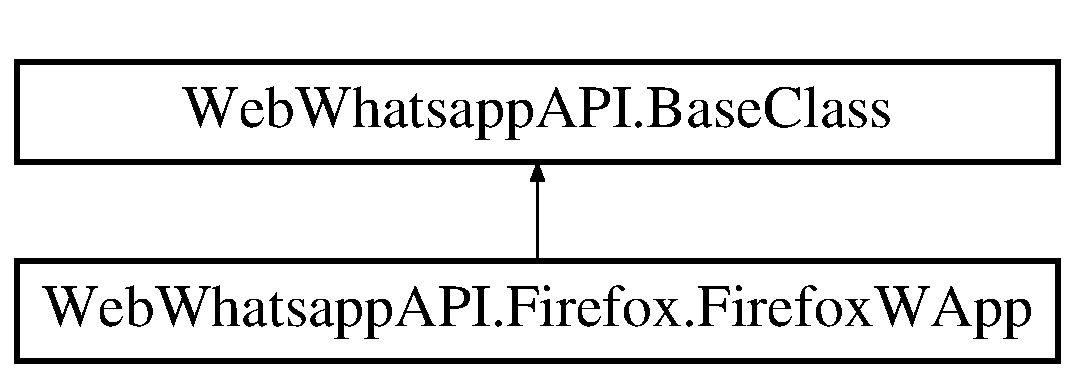
\includegraphics[height=2.000000cm]{class_web_whatsapp_a_p_i_1_1_base_class}
\end{center}
\end{figure}
\subsection*{Classes}
\begin{DoxyCompactItemize}
\item 
class \hyperlink{class_web_whatsapp_a_p_i_1_1_base_class_1_1_auto_save_settings}{Auto\+Save\+Settings}
\begin{DoxyCompactList}\small\item\em The save settings of the an driver \end{DoxyCompactList}\item 
class \hyperlink{class_web_whatsapp_a_p_i_1_1_base_class_1_1_chat_settings}{Chat\+Settings}
\begin{DoxyCompactList}\small\item\em The settings of the an driver \end{DoxyCompactList}\item 
class \hyperlink{class_web_whatsapp_a_p_i_1_1_base_class_1_1_msg_args}{Msg\+Args}
\begin{DoxyCompactList}\small\item\em Arguments used by Msg event \end{DoxyCompactList}\end{DoxyCompactItemize}
\subsection*{Public Member Functions}
\begin{DoxyCompactItemize}
\item 
\mbox{\Hypertarget{class_web_whatsapp_a_p_i_1_1_base_class_a33f2d663d89b991fead5ff2aba0dbc3c}\label{class_web_whatsapp_a_p_i_1_1_base_class_a33f2d663d89b991fead5ff2aba0dbc3c}} 
delegate void {\bfseries Msg\+Recieved\+Event\+Handler} (\hyperlink{class_web_whatsapp_a_p_i_1_1_base_class_1_1_msg_args}{Msg\+Args} e)
\item 
bool \hyperlink{class_web_whatsapp_a_p_i_1_1_base_class_ace95215a9d65215e30c8fe3582800878}{On\+Login\+Page} ()
\begin{DoxyCompactList}\small\item\em Returns if the Login page and QR has loaded \end{DoxyCompactList}\item 
bool \hyperlink{class_web_whatsapp_a_p_i_1_1_base_class_a8784fc769ca33afbbdb7478f0998de19}{Is\+Phone\+Connected} ()
\begin{DoxyCompactList}\small\item\em Check\textquotesingle{}s if we get the notification \char`\"{}\+Phone\+Not\+Connected\char`\"{} \end{DoxyCompactList}\item 
string \hyperlink{class_web_whatsapp_a_p_i_1_1_base_class_ad181052c89c24e15d53aa81c1afe531c}{Get\+Q\+R\+Image\+R\+AW} ()
\begin{DoxyCompactList}\small\item\em Gets raw QR string \end{DoxyCompactList}\item 
Image \hyperlink{class_web_whatsapp_a_p_i_1_1_base_class_ac9738e95307e38b1ef493c1164edb60c}{Get\+Q\+R\+Image} ()
\begin{DoxyCompactList}\small\item\em Gets an C\# image of the QR on the homepage \end{DoxyCompactList}\item 
async Task \hyperlink{class_web_whatsapp_a_p_i_1_1_base_class_a1da111623bfd6bee9401b049560e2646}{Message\+Scanner} ()
\begin{DoxyCompactList}\small\item\em Checks for messages which enables On\+Msg\+Recieved event \end{DoxyCompactList}\item 
virtual void \hyperlink{class_web_whatsapp_a_p_i_1_1_base_class_aaa7e5947e31c9f475c95c9818f6c3a00}{Start\+Driver} (I\+Web\+Driver driver, string savefile)
\begin{DoxyCompactList}\small\item\em Starts selenium driver, while loading a save file Note\+: these functions don\textquotesingle{}t make drivers \end{DoxyCompactList}\item 
virtual void \hyperlink{class_web_whatsapp_a_p_i_1_1_base_class_a8108d46b4176fc74fb49626e8122df88}{Start\+Driver} ()
\begin{DoxyCompactList}\small\item\em Starts selenium driver(only really used internally or virtually) Note\+: these functions don\textquotesingle{}t make drivers \end{DoxyCompactList}\item 
virtual void \hyperlink{class_web_whatsapp_a_p_i_1_1_base_class_a3a26ad50a4ba508f1162402bc00e128b}{Start\+Driver} (I\+Web\+Driver driver)
\begin{DoxyCompactList}\small\item\em Starts selenium driver Note\+: these functions don\textquotesingle{}t make drivers \end{DoxyCompactList}\item 
virtual void \hyperlink{class_web_whatsapp_a_p_i_1_1_base_class_a03ddf85cb437ebabb7f3444d856bd8a7}{Save} (string File\+Name)
\begin{DoxyCompactList}\small\item\em Saves settings and more to file \end{DoxyCompactList}\item 
virtual void \hyperlink{class_web_whatsapp_a_p_i_1_1_base_class_a6e8b8b0fbf62bffb3e153f4003280626}{Load} (string File\+Name)
\begin{DoxyCompactList}\small\item\em Loads a file containing Settings and cookies \end{DoxyCompactList}\item 
string \hyperlink{class_web_whatsapp_a_p_i_1_1_base_class_a9b62276c558e7e81cf507af854cdc0b2}{Get\+Lastest\+Text} (out string Pname)
\begin{DoxyCompactList}\small\item\em Gets the latest test \end{DoxyCompactList}\item 
void \hyperlink{class_web_whatsapp_a_p_i_1_1_base_class_a394d26a4172531e8149b5e084917dc99}{Send\+Message} (string message, string person=null)
\begin{DoxyCompactList}\small\item\em Send message to person \end{DoxyCompactList}\end{DoxyCompactItemize}
\subsection*{Public Attributes}
\begin{DoxyCompactItemize}
\item 
\hyperlink{class_web_whatsapp_a_p_i_1_1_base_class_1_1_chat_settings}{Chat\+Settings} \hyperlink{class_web_whatsapp_a_p_i_1_1_base_class_af7b5c73d834b7c97f6aa1947310af34e}{settings} = new \hyperlink{class_web_whatsapp_a_p_i_1_1_base_class_1_1_chat_settings}{Chat\+Settings}()
\begin{DoxyCompactList}\small\item\em Current settings \end{DoxyCompactList}\end{DoxyCompactItemize}
\subsection*{Protected Member Functions}
\begin{DoxyCompactItemize}
\item 
\mbox{\Hypertarget{class_web_whatsapp_a_p_i_1_1_base_class_a797576c847b00eee08dd92693bd522c4}\label{class_web_whatsapp_a_p_i_1_1_base_class_a797576c847b00eee08dd92693bd522c4}} 
void {\bfseries Raise\+\_\+\+Recieved\+Message} (string Msg, string Sender)
\item 
Image \hyperlink{class_web_whatsapp_a_p_i_1_1_base_class_a3c18dac86c5b0a57ebfb1822e89518d8}{Base64\+To\+Image} (string base64\+String)
\begin{DoxyCompactList}\small\item\em \href{https://stackoverflow.com/a/18827264}{\tt https\+://stackoverflow.\+com/a/18827264} \end{DoxyCompactList}\item 
virtual void \hyperlink{class_web_whatsapp_a_p_i_1_1_base_class_a56a2f1cfc0bef6cad2aae521e9c4d20a}{Auto\+Save} ()
\begin{DoxyCompactList}\small\item\em Saves to file \end{DoxyCompactList}\item 
void \hyperlink{class_web_whatsapp_a_p_i_1_1_base_class_a69c20548bf1e5d5e2ed200f6d44222e5}{Has\+Started\+Check} (bool Invert=false)
\begin{DoxyCompactList}\small\item\em only for internal use; throws exception if the driver has already started(can be inverted) \end{DoxyCompactList}\end{DoxyCompactItemize}
\subsection*{Protected Attributes}
\begin{DoxyCompactItemize}
\item 
\mbox{\Hypertarget{class_web_whatsapp_a_p_i_1_1_base_class_a2887b40fd1edaad98a26848369f83864}\label{class_web_whatsapp_a_p_i_1_1_base_class_a2887b40fd1edaad98a26848369f83864}} 
I\+Web\+Driver {\bfseries driver} = null
\item 
\mbox{\Hypertarget{class_web_whatsapp_a_p_i_1_1_base_class_a10068a3275629827584bda048227c456}\label{class_web_whatsapp_a_p_i_1_1_base_class_a10068a3275629827584bda048227c456}} 
Event\+Firing\+Web\+Driver {\bfseries event\+Driver} = null
\end{DoxyCompactItemize}
\subsection*{Properties}
\begin{DoxyCompactItemize}
\item 
\mbox{\Hypertarget{class_web_whatsapp_a_p_i_1_1_base_class_ac579478d77363feb4ffde2e9bcf48c21}\label{class_web_whatsapp_a_p_i_1_1_base_class_ac579478d77363feb4ffde2e9bcf48c21}} 
bool {\bfseries Has\+Started}\hspace{0.3cm}{\ttfamily  \mbox{[}get, protected set\mbox{]}}
\item 
I\+Web\+Driver \hyperlink{class_web_whatsapp_a_p_i_1_1_base_class_afc0c364092139747b980a1ad6b1e2321}{Web\+Driver}\hspace{0.3cm}{\ttfamily  \mbox{[}get\mbox{]}}
\begin{DoxyCompactList}\small\item\em A refrence to the Selenium Web\+Driver used; Selenium.\+Web\+Driver required \end{DoxyCompactList}\item 
Event\+Firing\+Web\+Driver \hyperlink{class_web_whatsapp_a_p_i_1_1_base_class_a1db62394318cea6839e32f2820fb426f}{Event\+Driver}\hspace{0.3cm}{\ttfamily  \mbox{[}get\mbox{]}}
\begin{DoxyCompactList}\small\item\em An event Web\+Driver from selenium; Selenium.\+Support package required \end{DoxyCompactList}\end{DoxyCompactItemize}
\subsection*{Events}
\begin{DoxyCompactItemize}
\item 
\mbox{\Hypertarget{class_web_whatsapp_a_p_i_1_1_base_class_a5baefb689c909b3db1816d274ea9596b}\label{class_web_whatsapp_a_p_i_1_1_base_class_a5baefb689c909b3db1816d274ea9596b}} 
Msg\+Recieved\+Event\+Handler {\bfseries On\+Msg\+Recieved}
\end{DoxyCompactItemize}


\subsection{Member Function Documentation}
\mbox{\Hypertarget{class_web_whatsapp_a_p_i_1_1_base_class_a56a2f1cfc0bef6cad2aae521e9c4d20a}\label{class_web_whatsapp_a_p_i_1_1_base_class_a56a2f1cfc0bef6cad2aae521e9c4d20a}} 
\index{Web\+Whatsapp\+A\+P\+I\+::\+Base\+Class@{Web\+Whatsapp\+A\+P\+I\+::\+Base\+Class}!Auto\+Save@{Auto\+Save}}
\index{Auto\+Save@{Auto\+Save}!Web\+Whatsapp\+A\+P\+I\+::\+Base\+Class@{Web\+Whatsapp\+A\+P\+I\+::\+Base\+Class}}
\subsubsection{\texorpdfstring{Auto\+Save()}{AutoSave()}}
{\footnotesize\ttfamily virtual void Web\+Whatsapp\+A\+P\+I.\+Base\+Class.\+Auto\+Save (\begin{DoxyParamCaption}{ }\end{DoxyParamCaption})\hspace{0.3cm}{\ttfamily [inline]}, {\ttfamily [protected]}, {\ttfamily [virtual]}}



Saves to file 

\mbox{\Hypertarget{class_web_whatsapp_a_p_i_1_1_base_class_a3c18dac86c5b0a57ebfb1822e89518d8}\label{class_web_whatsapp_a_p_i_1_1_base_class_a3c18dac86c5b0a57ebfb1822e89518d8}} 
\index{Web\+Whatsapp\+A\+P\+I\+::\+Base\+Class@{Web\+Whatsapp\+A\+P\+I\+::\+Base\+Class}!Base64\+To\+Image@{Base64\+To\+Image}}
\index{Base64\+To\+Image@{Base64\+To\+Image}!Web\+Whatsapp\+A\+P\+I\+::\+Base\+Class@{Web\+Whatsapp\+A\+P\+I\+::\+Base\+Class}}
\subsubsection{\texorpdfstring{Base64\+To\+Image()}{Base64ToImage()}}
{\footnotesize\ttfamily Image Web\+Whatsapp\+A\+P\+I.\+Base\+Class.\+Base64\+To\+Image (\begin{DoxyParamCaption}\item[{string}]{base64\+String }\end{DoxyParamCaption})\hspace{0.3cm}{\ttfamily [inline]}, {\ttfamily [protected]}}



\href{https://stackoverflow.com/a/18827264}{\tt https\+://stackoverflow.\+com/a/18827264} 


\begin{DoxyParams}{Parameters}
{\em base64\+String} & Base 64 string\\
\hline
\end{DoxyParams}
\begin{DoxyReturn}{Returns}
an image
\end{DoxyReturn}
\mbox{\Hypertarget{class_web_whatsapp_a_p_i_1_1_base_class_a9b62276c558e7e81cf507af854cdc0b2}\label{class_web_whatsapp_a_p_i_1_1_base_class_a9b62276c558e7e81cf507af854cdc0b2}} 
\index{Web\+Whatsapp\+A\+P\+I\+::\+Base\+Class@{Web\+Whatsapp\+A\+P\+I\+::\+Base\+Class}!Get\+Lastest\+Text@{Get\+Lastest\+Text}}
\index{Get\+Lastest\+Text@{Get\+Lastest\+Text}!Web\+Whatsapp\+A\+P\+I\+::\+Base\+Class@{Web\+Whatsapp\+A\+P\+I\+::\+Base\+Class}}
\subsubsection{\texorpdfstring{Get\+Lastest\+Text()}{GetLastestText()}}
{\footnotesize\ttfamily string Web\+Whatsapp\+A\+P\+I.\+Base\+Class.\+Get\+Lastest\+Text (\begin{DoxyParamCaption}\item[{out string}]{Pname }\end{DoxyParamCaption})\hspace{0.3cm}{\ttfamily [inline]}}



Gets the latest test 


\begin{DoxyParams}{Parameters}
{\em Pname} & \mbox{[}Optional output\mbox{]} the person that send the message\\
\hline
\end{DoxyParams}
\begin{DoxyReturn}{Returns}

\end{DoxyReturn}
\mbox{\Hypertarget{class_web_whatsapp_a_p_i_1_1_base_class_ac9738e95307e38b1ef493c1164edb60c}\label{class_web_whatsapp_a_p_i_1_1_base_class_ac9738e95307e38b1ef493c1164edb60c}} 
\index{Web\+Whatsapp\+A\+P\+I\+::\+Base\+Class@{Web\+Whatsapp\+A\+P\+I\+::\+Base\+Class}!Get\+Q\+R\+Image@{Get\+Q\+R\+Image}}
\index{Get\+Q\+R\+Image@{Get\+Q\+R\+Image}!Web\+Whatsapp\+A\+P\+I\+::\+Base\+Class@{Web\+Whatsapp\+A\+P\+I\+::\+Base\+Class}}
\subsubsection{\texorpdfstring{Get\+Q\+R\+Image()}{GetQRImage()}}
{\footnotesize\ttfamily Image Web\+Whatsapp\+A\+P\+I.\+Base\+Class.\+Get\+Q\+R\+Image (\begin{DoxyParamCaption}{ }\end{DoxyParamCaption})\hspace{0.3cm}{\ttfamily [inline]}}



Gets an C\# image of the QR on the homepage 

\begin{DoxyReturn}{Returns}
QR image; returns null if not available
\end{DoxyReturn}
\mbox{\Hypertarget{class_web_whatsapp_a_p_i_1_1_base_class_ad181052c89c24e15d53aa81c1afe531c}\label{class_web_whatsapp_a_p_i_1_1_base_class_ad181052c89c24e15d53aa81c1afe531c}} 
\index{Web\+Whatsapp\+A\+P\+I\+::\+Base\+Class@{Web\+Whatsapp\+A\+P\+I\+::\+Base\+Class}!Get\+Q\+R\+Image\+R\+AW@{Get\+Q\+R\+Image\+R\+AW}}
\index{Get\+Q\+R\+Image\+R\+AW@{Get\+Q\+R\+Image\+R\+AW}!Web\+Whatsapp\+A\+P\+I\+::\+Base\+Class@{Web\+Whatsapp\+A\+P\+I\+::\+Base\+Class}}
\subsubsection{\texorpdfstring{Get\+Q\+R\+Image\+R\+A\+W()}{GetQRImageRAW()}}
{\footnotesize\ttfamily string Web\+Whatsapp\+A\+P\+I.\+Base\+Class.\+Get\+Q\+R\+Image\+R\+AW (\begin{DoxyParamCaption}{ }\end{DoxyParamCaption})\hspace{0.3cm}{\ttfamily [inline]}}



Gets raw QR string 

\begin{DoxyReturn}{Returns}
sting(base64) of the image; returns null if not available
\end{DoxyReturn}
\mbox{\Hypertarget{class_web_whatsapp_a_p_i_1_1_base_class_a69c20548bf1e5d5e2ed200f6d44222e5}\label{class_web_whatsapp_a_p_i_1_1_base_class_a69c20548bf1e5d5e2ed200f6d44222e5}} 
\index{Web\+Whatsapp\+A\+P\+I\+::\+Base\+Class@{Web\+Whatsapp\+A\+P\+I\+::\+Base\+Class}!Has\+Started\+Check@{Has\+Started\+Check}}
\index{Has\+Started\+Check@{Has\+Started\+Check}!Web\+Whatsapp\+A\+P\+I\+::\+Base\+Class@{Web\+Whatsapp\+A\+P\+I\+::\+Base\+Class}}
\subsubsection{\texorpdfstring{Has\+Started\+Check()}{HasStartedCheck()}}
{\footnotesize\ttfamily void Web\+Whatsapp\+A\+P\+I.\+Base\+Class.\+Has\+Started\+Check (\begin{DoxyParamCaption}\item[{bool}]{Invert = {\ttfamily false} }\end{DoxyParamCaption})\hspace{0.3cm}{\ttfamily [inline]}, {\ttfamily [protected]}}



only for internal use; throws exception if the driver has already started(can be inverted) 

\mbox{\Hypertarget{class_web_whatsapp_a_p_i_1_1_base_class_a8784fc769ca33afbbdb7478f0998de19}\label{class_web_whatsapp_a_p_i_1_1_base_class_a8784fc769ca33afbbdb7478f0998de19}} 
\index{Web\+Whatsapp\+A\+P\+I\+::\+Base\+Class@{Web\+Whatsapp\+A\+P\+I\+::\+Base\+Class}!Is\+Phone\+Connected@{Is\+Phone\+Connected}}
\index{Is\+Phone\+Connected@{Is\+Phone\+Connected}!Web\+Whatsapp\+A\+P\+I\+::\+Base\+Class@{Web\+Whatsapp\+A\+P\+I\+::\+Base\+Class}}
\subsubsection{\texorpdfstring{Is\+Phone\+Connected()}{IsPhoneConnected()}}
{\footnotesize\ttfamily bool Web\+Whatsapp\+A\+P\+I.\+Base\+Class.\+Is\+Phone\+Connected (\begin{DoxyParamCaption}{ }\end{DoxyParamCaption})\hspace{0.3cm}{\ttfamily [inline]}}



Check\textquotesingle{}s if we get the notification \char`\"{}\+Phone\+Not\+Connected\char`\"{} 

\begin{DoxyReturn}{Returns}
bool; true if connected
\end{DoxyReturn}
\mbox{\Hypertarget{class_web_whatsapp_a_p_i_1_1_base_class_a6e8b8b0fbf62bffb3e153f4003280626}\label{class_web_whatsapp_a_p_i_1_1_base_class_a6e8b8b0fbf62bffb3e153f4003280626}} 
\index{Web\+Whatsapp\+A\+P\+I\+::\+Base\+Class@{Web\+Whatsapp\+A\+P\+I\+::\+Base\+Class}!Load@{Load}}
\index{Load@{Load}!Web\+Whatsapp\+A\+P\+I\+::\+Base\+Class@{Web\+Whatsapp\+A\+P\+I\+::\+Base\+Class}}
\subsubsection{\texorpdfstring{Load()}{Load()}}
{\footnotesize\ttfamily virtual void Web\+Whatsapp\+A\+P\+I.\+Base\+Class.\+Load (\begin{DoxyParamCaption}\item[{string}]{File\+Name }\end{DoxyParamCaption})\hspace{0.3cm}{\ttfamily [inline]}, {\ttfamily [virtual]}}



Loads a file containing Settings and cookies 


\begin{DoxyParams}{Parameters}
{\em File\+Name} & path to Filename\\
\hline
\end{DoxyParams}
\mbox{\Hypertarget{class_web_whatsapp_a_p_i_1_1_base_class_a1da111623bfd6bee9401b049560e2646}\label{class_web_whatsapp_a_p_i_1_1_base_class_a1da111623bfd6bee9401b049560e2646}} 
\index{Web\+Whatsapp\+A\+P\+I\+::\+Base\+Class@{Web\+Whatsapp\+A\+P\+I\+::\+Base\+Class}!Message\+Scanner@{Message\+Scanner}}
\index{Message\+Scanner@{Message\+Scanner}!Web\+Whatsapp\+A\+P\+I\+::\+Base\+Class@{Web\+Whatsapp\+A\+P\+I\+::\+Base\+Class}}
\subsubsection{\texorpdfstring{Message\+Scanner()}{MessageScanner()}}
{\footnotesize\ttfamily async Task Web\+Whatsapp\+A\+P\+I.\+Base\+Class.\+Message\+Scanner (\begin{DoxyParamCaption}{ }\end{DoxyParamCaption})\hspace{0.3cm}{\ttfamily [inline]}}



Checks for messages which enables On\+Msg\+Recieved event 

\begin{DoxyReturn}{Returns}
Nothing
\end{DoxyReturn}
\mbox{\Hypertarget{class_web_whatsapp_a_p_i_1_1_base_class_ace95215a9d65215e30c8fe3582800878}\label{class_web_whatsapp_a_p_i_1_1_base_class_ace95215a9d65215e30c8fe3582800878}} 
\index{Web\+Whatsapp\+A\+P\+I\+::\+Base\+Class@{Web\+Whatsapp\+A\+P\+I\+::\+Base\+Class}!On\+Login\+Page@{On\+Login\+Page}}
\index{On\+Login\+Page@{On\+Login\+Page}!Web\+Whatsapp\+A\+P\+I\+::\+Base\+Class@{Web\+Whatsapp\+A\+P\+I\+::\+Base\+Class}}
\subsubsection{\texorpdfstring{On\+Login\+Page()}{OnLoginPage()}}
{\footnotesize\ttfamily bool Web\+Whatsapp\+A\+P\+I.\+Base\+Class.\+On\+Login\+Page (\begin{DoxyParamCaption}{ }\end{DoxyParamCaption})\hspace{0.3cm}{\ttfamily [inline]}}



Returns if the Login page and QR has loaded 

\begin{DoxyReturn}{Returns}

\end{DoxyReturn}
\mbox{\Hypertarget{class_web_whatsapp_a_p_i_1_1_base_class_a03ddf85cb437ebabb7f3444d856bd8a7}\label{class_web_whatsapp_a_p_i_1_1_base_class_a03ddf85cb437ebabb7f3444d856bd8a7}} 
\index{Web\+Whatsapp\+A\+P\+I\+::\+Base\+Class@{Web\+Whatsapp\+A\+P\+I\+::\+Base\+Class}!Save@{Save}}
\index{Save@{Save}!Web\+Whatsapp\+A\+P\+I\+::\+Base\+Class@{Web\+Whatsapp\+A\+P\+I\+::\+Base\+Class}}
\subsubsection{\texorpdfstring{Save()}{Save()}}
{\footnotesize\ttfamily virtual void Web\+Whatsapp\+A\+P\+I.\+Base\+Class.\+Save (\begin{DoxyParamCaption}\item[{string}]{File\+Name }\end{DoxyParamCaption})\hspace{0.3cm}{\ttfamily [inline]}, {\ttfamily [virtual]}}



Saves settings and more to file 


\begin{DoxyParams}{Parameters}
{\em File\+Name} & Path/\+Filename to make the file (e.\+g. save1.\+bin)\\
\hline
\end{DoxyParams}
\mbox{\Hypertarget{class_web_whatsapp_a_p_i_1_1_base_class_a394d26a4172531e8149b5e084917dc99}\label{class_web_whatsapp_a_p_i_1_1_base_class_a394d26a4172531e8149b5e084917dc99}} 
\index{Web\+Whatsapp\+A\+P\+I\+::\+Base\+Class@{Web\+Whatsapp\+A\+P\+I\+::\+Base\+Class}!Send\+Message@{Send\+Message}}
\index{Send\+Message@{Send\+Message}!Web\+Whatsapp\+A\+P\+I\+::\+Base\+Class@{Web\+Whatsapp\+A\+P\+I\+::\+Base\+Class}}
\subsubsection{\texorpdfstring{Send\+Message()}{SendMessage()}}
{\footnotesize\ttfamily void Web\+Whatsapp\+A\+P\+I.\+Base\+Class.\+Send\+Message (\begin{DoxyParamCaption}\item[{string}]{message,  }\item[{string}]{person = {\ttfamily null} }\end{DoxyParamCaption})\hspace{0.3cm}{\ttfamily [inline]}}



Send message to person 


\begin{DoxyParams}{Parameters}
{\em message} & string to send\\
\hline
{\em person} & person to send to (if null send to active)\\
\hline
\end{DoxyParams}
\mbox{\Hypertarget{class_web_whatsapp_a_p_i_1_1_base_class_aaa7e5947e31c9f475c95c9818f6c3a00}\label{class_web_whatsapp_a_p_i_1_1_base_class_aaa7e5947e31c9f475c95c9818f6c3a00}} 
\index{Web\+Whatsapp\+A\+P\+I\+::\+Base\+Class@{Web\+Whatsapp\+A\+P\+I\+::\+Base\+Class}!Start\+Driver@{Start\+Driver}}
\index{Start\+Driver@{Start\+Driver}!Web\+Whatsapp\+A\+P\+I\+::\+Base\+Class@{Web\+Whatsapp\+A\+P\+I\+::\+Base\+Class}}
\subsubsection{\texorpdfstring{Start\+Driver()}{StartDriver()}\hspace{0.1cm}{\footnotesize\ttfamily [1/3]}}
{\footnotesize\ttfamily virtual void Web\+Whatsapp\+A\+P\+I.\+Base\+Class.\+Start\+Driver (\begin{DoxyParamCaption}\item[{I\+Web\+Driver}]{driver,  }\item[{string}]{savefile }\end{DoxyParamCaption})\hspace{0.3cm}{\ttfamily [inline]}, {\ttfamily [virtual]}}



Starts selenium driver, while loading a save file Note\+: these functions don\textquotesingle{}t make drivers 


\begin{DoxyParams}{Parameters}
{\em driver} & The driver\\
\hline
{\em savefile} & Path to savefile\\
\hline
\end{DoxyParams}
\mbox{\Hypertarget{class_web_whatsapp_a_p_i_1_1_base_class_a8108d46b4176fc74fb49626e8122df88}\label{class_web_whatsapp_a_p_i_1_1_base_class_a8108d46b4176fc74fb49626e8122df88}} 
\index{Web\+Whatsapp\+A\+P\+I\+::\+Base\+Class@{Web\+Whatsapp\+A\+P\+I\+::\+Base\+Class}!Start\+Driver@{Start\+Driver}}
\index{Start\+Driver@{Start\+Driver}!Web\+Whatsapp\+A\+P\+I\+::\+Base\+Class@{Web\+Whatsapp\+A\+P\+I\+::\+Base\+Class}}
\subsubsection{\texorpdfstring{Start\+Driver()}{StartDriver()}\hspace{0.1cm}{\footnotesize\ttfamily [2/3]}}
{\footnotesize\ttfamily virtual void Web\+Whatsapp\+A\+P\+I.\+Base\+Class.\+Start\+Driver (\begin{DoxyParamCaption}{ }\end{DoxyParamCaption})\hspace{0.3cm}{\ttfamily [inline]}, {\ttfamily [virtual]}}



Starts selenium driver(only really used internally or virtually) Note\+: these functions don\textquotesingle{}t make drivers 



Reimplemented in \hyperlink{class_web_whatsapp_a_p_i_1_1_chrome_1_1_chrome_w_app_a2ed5da636b9baf0766bd6804739a9bfb}{Web\+Whatsapp\+A\+P\+I.\+Chrome.\+Chrome\+W\+App}, and \hyperlink{class_web_whatsapp_a_p_i_1_1_firefox_1_1_firefox_w_app_a80f406639e59bc4152b8f255962607f2}{Web\+Whatsapp\+A\+P\+I.\+Firefox.\+Firefox\+W\+App}.

\mbox{\Hypertarget{class_web_whatsapp_a_p_i_1_1_base_class_a3a26ad50a4ba508f1162402bc00e128b}\label{class_web_whatsapp_a_p_i_1_1_base_class_a3a26ad50a4ba508f1162402bc00e128b}} 
\index{Web\+Whatsapp\+A\+P\+I\+::\+Base\+Class@{Web\+Whatsapp\+A\+P\+I\+::\+Base\+Class}!Start\+Driver@{Start\+Driver}}
\index{Start\+Driver@{Start\+Driver}!Web\+Whatsapp\+A\+P\+I\+::\+Base\+Class@{Web\+Whatsapp\+A\+P\+I\+::\+Base\+Class}}
\subsubsection{\texorpdfstring{Start\+Driver()}{StartDriver()}\hspace{0.1cm}{\footnotesize\ttfamily [3/3]}}
{\footnotesize\ttfamily virtual void Web\+Whatsapp\+A\+P\+I.\+Base\+Class.\+Start\+Driver (\begin{DoxyParamCaption}\item[{I\+Web\+Driver}]{driver }\end{DoxyParamCaption})\hspace{0.3cm}{\ttfamily [inline]}, {\ttfamily [virtual]}}



Starts selenium driver Note\+: these functions don\textquotesingle{}t make drivers 


\begin{DoxyParams}{Parameters}
{\em driver} & The selenium driver\\
\hline
\end{DoxyParams}


\subsection{Member Data Documentation}
\mbox{\Hypertarget{class_web_whatsapp_a_p_i_1_1_base_class_af7b5c73d834b7c97f6aa1947310af34e}\label{class_web_whatsapp_a_p_i_1_1_base_class_af7b5c73d834b7c97f6aa1947310af34e}} 
\index{Web\+Whatsapp\+A\+P\+I\+::\+Base\+Class@{Web\+Whatsapp\+A\+P\+I\+::\+Base\+Class}!settings@{settings}}
\index{settings@{settings}!Web\+Whatsapp\+A\+P\+I\+::\+Base\+Class@{Web\+Whatsapp\+A\+P\+I\+::\+Base\+Class}}
\subsubsection{\texorpdfstring{settings}{settings}}
{\footnotesize\ttfamily \hyperlink{class_web_whatsapp_a_p_i_1_1_base_class_1_1_chat_settings}{Chat\+Settings} Web\+Whatsapp\+A\+P\+I.\+Base\+Class.\+settings = new \hyperlink{class_web_whatsapp_a_p_i_1_1_base_class_1_1_chat_settings}{Chat\+Settings}()}



Current settings 



\subsection{Property Documentation}
\mbox{\Hypertarget{class_web_whatsapp_a_p_i_1_1_base_class_a1db62394318cea6839e32f2820fb426f}\label{class_web_whatsapp_a_p_i_1_1_base_class_a1db62394318cea6839e32f2820fb426f}} 
\index{Web\+Whatsapp\+A\+P\+I\+::\+Base\+Class@{Web\+Whatsapp\+A\+P\+I\+::\+Base\+Class}!Event\+Driver@{Event\+Driver}}
\index{Event\+Driver@{Event\+Driver}!Web\+Whatsapp\+A\+P\+I\+::\+Base\+Class@{Web\+Whatsapp\+A\+P\+I\+::\+Base\+Class}}
\subsubsection{\texorpdfstring{Event\+Driver}{EventDriver}}
{\footnotesize\ttfamily Event\+Firing\+Web\+Driver Web\+Whatsapp\+A\+P\+I.\+Base\+Class.\+Event\+Driver\hspace{0.3cm}{\ttfamily [get]}}



An event Web\+Driver from selenium; Selenium.\+Support package required 

\mbox{\Hypertarget{class_web_whatsapp_a_p_i_1_1_base_class_afc0c364092139747b980a1ad6b1e2321}\label{class_web_whatsapp_a_p_i_1_1_base_class_afc0c364092139747b980a1ad6b1e2321}} 
\index{Web\+Whatsapp\+A\+P\+I\+::\+Base\+Class@{Web\+Whatsapp\+A\+P\+I\+::\+Base\+Class}!Web\+Driver@{Web\+Driver}}
\index{Web\+Driver@{Web\+Driver}!Web\+Whatsapp\+A\+P\+I\+::\+Base\+Class@{Web\+Whatsapp\+A\+P\+I\+::\+Base\+Class}}
\subsubsection{\texorpdfstring{Web\+Driver}{WebDriver}}
{\footnotesize\ttfamily I\+Web\+Driver Web\+Whatsapp\+A\+P\+I.\+Base\+Class.\+Web\+Driver\hspace{0.3cm}{\ttfamily [get]}}



A refrence to the Selenium Web\+Driver used; Selenium.\+Web\+Driver required 



The documentation for this class was generated from the following file\+:\begin{DoxyCompactItemize}
\item 
Web\+Whatsapp\+A\+P\+I/Base\+Class.\+cs\end{DoxyCompactItemize}

\hypertarget{class_web_whatsapp_a_p_i_1_1_base_class_1_1_chat_settings}{}\section{Web\+Whatsapp\+A\+P\+I.\+Base\+Class.\+Chat\+Settings Class Reference}
\label{class_web_whatsapp_a_p_i_1_1_base_class_1_1_chat_settings}\index{Web\+Whatsapp\+A\+P\+I.\+Base\+Class.\+Chat\+Settings@{Web\+Whatsapp\+A\+P\+I.\+Base\+Class.\+Chat\+Settings}}


The settings of the an driver  


\subsection*{Public Attributes}
\begin{DoxyCompactItemize}
\item 
\mbox{\Hypertarget{class_web_whatsapp_a_p_i_1_1_base_class_1_1_chat_settings_ae5a3f25d99ac2fe65071e6ce7ded3a42}\label{class_web_whatsapp_a_p_i_1_1_base_class_1_1_chat_settings_ae5a3f25d99ac2fe65071e6ce7ded3a42}} 
bool {\bfseries Allow\+G\+ET} = true
\item 
\mbox{\Hypertarget{class_web_whatsapp_a_p_i_1_1_base_class_1_1_chat_settings_aedbc99082538d5a61c653caa7e336e1c}\label{class_web_whatsapp_a_p_i_1_1_base_class_1_1_chat_settings_aedbc99082538d5a61c653caa7e336e1c}} 
bool {\bfseries Auto\+Save\+Settings} = true
\item 
\mbox{\Hypertarget{class_web_whatsapp_a_p_i_1_1_base_class_1_1_chat_settings_a0cbc84fe0f8fae01e324a6184c31dd65}\label{class_web_whatsapp_a_p_i_1_1_base_class_1_1_chat_settings_a0cbc84fe0f8fae01e324a6184c31dd65}} 
bool {\bfseries Save\+Messages} = false
\item 
\mbox{\Hypertarget{class_web_whatsapp_a_p_i_1_1_base_class_1_1_chat_settings_ae56212dc2d8c5532b446368ddc828b92}\label{class_web_whatsapp_a_p_i_1_1_base_class_1_1_chat_settings_ae56212dc2d8c5532b446368ddc828b92}} 
\hyperlink{class_web_whatsapp_a_p_i_1_1_base_class_1_1_auto_save_settings}{Auto\+Save\+Settings} {\bfseries Save\+Settings} = new \hyperlink{class_web_whatsapp_a_p_i_1_1_base_class_1_1_auto_save_settings}{Auto\+Save\+Settings}()
\end{DoxyCompactItemize}


\subsection{Detailed Description}
The settings of the an driver 



The documentation for this class was generated from the following file\+:\begin{DoxyCompactItemize}
\item 
Web\+Whatsapp\+A\+P\+I/Base\+Class.\+cs\end{DoxyCompactItemize}

\hypertarget{class_web_whatsapp_a_p_i_1_1_chrome_1_1_chrome_w_app}{}\section{Web\+Whatsapp\+A\+P\+I.\+Chrome.\+Chrome\+W\+App Class Reference}
\label{class_web_whatsapp_a_p_i_1_1_chrome_1_1_chrome_w_app}\index{Web\+Whatsapp\+A\+P\+I.\+Chrome.\+Chrome\+W\+App@{Web\+Whatsapp\+A\+P\+I.\+Chrome.\+Chrome\+W\+App}}
Inheritance diagram for Web\+Whatsapp\+A\+P\+I.\+Chrome.\+Chrome\+W\+App\+:\begin{figure}[H]
\begin{center}
\leavevmode
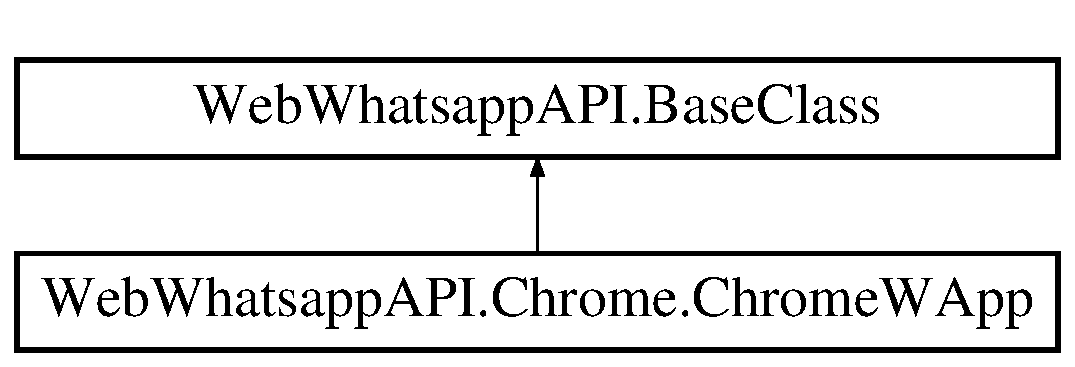
\includegraphics[height=2.000000cm]{class_web_whatsapp_a_p_i_1_1_chrome_1_1_chrome_w_app}
\end{center}
\end{figure}
\subsection*{Public Member Functions}
\begin{DoxyCompactItemize}
\item 
\hyperlink{class_web_whatsapp_a_p_i_1_1_chrome_1_1_chrome_w_app_a9c8ebf61ff410da72e8a50d68cbcf0f5}{Chrome\+W\+App} ()
\begin{DoxyCompactList}\small\item\em Make a new Chrome\+Whatsapp Instance \end{DoxyCompactList}\item 
override void \hyperlink{class_web_whatsapp_a_p_i_1_1_chrome_1_1_chrome_w_app_a2ed5da636b9baf0766bd6804739a9bfb}{Start\+Driver} ()
\begin{DoxyCompactList}\small\item\em Starts the chrome driver with settings \end{DoxyCompactList}\item 
void \hyperlink{class_web_whatsapp_a_p_i_1_1_chrome_1_1_chrome_w_app_aaf4df519b4cda569bbb8f6d757a372f2}{Add\+Extension} (string path)
\begin{DoxyCompactList}\small\item\em Adds an extension Note\+: has to be before start of driver \end{DoxyCompactList}\item 
void \hyperlink{class_web_whatsapp_a_p_i_1_1_chrome_1_1_chrome_w_app_a6a01da1da6329da843cbed002716ea36}{Add\+Extension\+Base64} (string base64)
\begin{DoxyCompactList}\small\item\em Adds an base64 encoded extension Note\+: has to be before start of driver \end{DoxyCompactList}\item 
void \hyperlink{class_web_whatsapp_a_p_i_1_1_chrome_1_1_chrome_w_app_a4dd7c9e90b65a5c3fdbb7d0b12f4823c}{Add\+Start\+Argument} (string arg)
\begin{DoxyCompactList}\small\item\em Adds an argument when chrome is started Note\+: has to be before start of driver \end{DoxyCompactList}\end{DoxyCompactItemize}
\subsection*{Additional Inherited Members}


\subsection{Constructor \& Destructor Documentation}
\mbox{\Hypertarget{class_web_whatsapp_a_p_i_1_1_chrome_1_1_chrome_w_app_a9c8ebf61ff410da72e8a50d68cbcf0f5}\label{class_web_whatsapp_a_p_i_1_1_chrome_1_1_chrome_w_app_a9c8ebf61ff410da72e8a50d68cbcf0f5}} 
\index{Web\+Whatsapp\+A\+P\+I\+::\+Chrome\+::\+Chrome\+W\+App@{Web\+Whatsapp\+A\+P\+I\+::\+Chrome\+::\+Chrome\+W\+App}!Chrome\+W\+App@{Chrome\+W\+App}}
\index{Chrome\+W\+App@{Chrome\+W\+App}!Web\+Whatsapp\+A\+P\+I\+::\+Chrome\+::\+Chrome\+W\+App@{Web\+Whatsapp\+A\+P\+I\+::\+Chrome\+::\+Chrome\+W\+App}}
\subsubsection{\texorpdfstring{Chrome\+W\+App()}{ChromeWApp()}}
{\footnotesize\ttfamily Web\+Whatsapp\+A\+P\+I.\+Chrome.\+Chrome\+W\+App.\+Chrome\+W\+App (\begin{DoxyParamCaption}{ }\end{DoxyParamCaption})\hspace{0.3cm}{\ttfamily [inline]}}



Make a new Chrome\+Whatsapp Instance 



\subsection{Member Function Documentation}
\mbox{\Hypertarget{class_web_whatsapp_a_p_i_1_1_chrome_1_1_chrome_w_app_aaf4df519b4cda569bbb8f6d757a372f2}\label{class_web_whatsapp_a_p_i_1_1_chrome_1_1_chrome_w_app_aaf4df519b4cda569bbb8f6d757a372f2}} 
\index{Web\+Whatsapp\+A\+P\+I\+::\+Chrome\+::\+Chrome\+W\+App@{Web\+Whatsapp\+A\+P\+I\+::\+Chrome\+::\+Chrome\+W\+App}!Add\+Extension@{Add\+Extension}}
\index{Add\+Extension@{Add\+Extension}!Web\+Whatsapp\+A\+P\+I\+::\+Chrome\+::\+Chrome\+W\+App@{Web\+Whatsapp\+A\+P\+I\+::\+Chrome\+::\+Chrome\+W\+App}}
\subsubsection{\texorpdfstring{Add\+Extension()}{AddExtension()}}
{\footnotesize\ttfamily void Web\+Whatsapp\+A\+P\+I.\+Chrome.\+Chrome\+W\+App.\+Add\+Extension (\begin{DoxyParamCaption}\item[{string}]{path }\end{DoxyParamCaption})\hspace{0.3cm}{\ttfamily [inline]}}



Adds an extension Note\+: has to be before start of driver 


\begin{DoxyParams}{Parameters}
{\em path} & \\
\hline
\end{DoxyParams}
\mbox{\Hypertarget{class_web_whatsapp_a_p_i_1_1_chrome_1_1_chrome_w_app_a6a01da1da6329da843cbed002716ea36}\label{class_web_whatsapp_a_p_i_1_1_chrome_1_1_chrome_w_app_a6a01da1da6329da843cbed002716ea36}} 
\index{Web\+Whatsapp\+A\+P\+I\+::\+Chrome\+::\+Chrome\+W\+App@{Web\+Whatsapp\+A\+P\+I\+::\+Chrome\+::\+Chrome\+W\+App}!Add\+Extension\+Base64@{Add\+Extension\+Base64}}
\index{Add\+Extension\+Base64@{Add\+Extension\+Base64}!Web\+Whatsapp\+A\+P\+I\+::\+Chrome\+::\+Chrome\+W\+App@{Web\+Whatsapp\+A\+P\+I\+::\+Chrome\+::\+Chrome\+W\+App}}
\subsubsection{\texorpdfstring{Add\+Extension\+Base64()}{AddExtensionBase64()}}
{\footnotesize\ttfamily void Web\+Whatsapp\+A\+P\+I.\+Chrome.\+Chrome\+W\+App.\+Add\+Extension\+Base64 (\begin{DoxyParamCaption}\item[{string}]{base64 }\end{DoxyParamCaption})\hspace{0.3cm}{\ttfamily [inline]}}



Adds an base64 encoded extension Note\+: has to be before start of driver 


\begin{DoxyParams}{Parameters}
{\em base64} & the extension\\
\hline
\end{DoxyParams}
\mbox{\Hypertarget{class_web_whatsapp_a_p_i_1_1_chrome_1_1_chrome_w_app_a4dd7c9e90b65a5c3fdbb7d0b12f4823c}\label{class_web_whatsapp_a_p_i_1_1_chrome_1_1_chrome_w_app_a4dd7c9e90b65a5c3fdbb7d0b12f4823c}} 
\index{Web\+Whatsapp\+A\+P\+I\+::\+Chrome\+::\+Chrome\+W\+App@{Web\+Whatsapp\+A\+P\+I\+::\+Chrome\+::\+Chrome\+W\+App}!Add\+Start\+Argument@{Add\+Start\+Argument}}
\index{Add\+Start\+Argument@{Add\+Start\+Argument}!Web\+Whatsapp\+A\+P\+I\+::\+Chrome\+::\+Chrome\+W\+App@{Web\+Whatsapp\+A\+P\+I\+::\+Chrome\+::\+Chrome\+W\+App}}
\subsubsection{\texorpdfstring{Add\+Start\+Argument()}{AddStartArgument()}}
{\footnotesize\ttfamily void Web\+Whatsapp\+A\+P\+I.\+Chrome.\+Chrome\+W\+App.\+Add\+Start\+Argument (\begin{DoxyParamCaption}\item[{string}]{arg }\end{DoxyParamCaption})\hspace{0.3cm}{\ttfamily [inline]}}



Adds an argument when chrome is started Note\+: has to be before start of driver 


\begin{DoxyParams}{Parameters}
{\em arg} & the argument\\
\hline
\end{DoxyParams}
\mbox{\Hypertarget{class_web_whatsapp_a_p_i_1_1_chrome_1_1_chrome_w_app_a2ed5da636b9baf0766bd6804739a9bfb}\label{class_web_whatsapp_a_p_i_1_1_chrome_1_1_chrome_w_app_a2ed5da636b9baf0766bd6804739a9bfb}} 
\index{Web\+Whatsapp\+A\+P\+I\+::\+Chrome\+::\+Chrome\+W\+App@{Web\+Whatsapp\+A\+P\+I\+::\+Chrome\+::\+Chrome\+W\+App}!Start\+Driver@{Start\+Driver}}
\index{Start\+Driver@{Start\+Driver}!Web\+Whatsapp\+A\+P\+I\+::\+Chrome\+::\+Chrome\+W\+App@{Web\+Whatsapp\+A\+P\+I\+::\+Chrome\+::\+Chrome\+W\+App}}
\subsubsection{\texorpdfstring{Start\+Driver()}{StartDriver()}}
{\footnotesize\ttfamily override void Web\+Whatsapp\+A\+P\+I.\+Chrome.\+Chrome\+W\+App.\+Start\+Driver (\begin{DoxyParamCaption}{ }\end{DoxyParamCaption})\hspace{0.3cm}{\ttfamily [inline]}, {\ttfamily [virtual]}}



Starts the chrome driver with settings 



Reimplemented from \hyperlink{class_web_whatsapp_a_p_i_1_1_base_class_a8108d46b4176fc74fb49626e8122df88}{Web\+Whatsapp\+A\+P\+I.\+Base\+Class}.



The documentation for this class was generated from the following file\+:\begin{DoxyCompactItemize}
\item 
Web\+Whatsapp\+A\+P\+I/Chrome.\+cs\end{DoxyCompactItemize}

\hypertarget{class_web_whatsapp_a_p_i_1_1_firefox_1_1_firefox_w_app}{}\section{Web\+Whatsapp\+A\+P\+I.\+Firefox.\+Firefox\+W\+App Class Reference}
\label{class_web_whatsapp_a_p_i_1_1_firefox_1_1_firefox_w_app}\index{Web\+Whatsapp\+A\+P\+I.\+Firefox.\+Firefox\+W\+App@{Web\+Whatsapp\+A\+P\+I.\+Firefox.\+Firefox\+W\+App}}
Inheritance diagram for Web\+Whatsapp\+A\+P\+I.\+Firefox.\+Firefox\+W\+App\+:\begin{figure}[H]
\begin{center}
\leavevmode
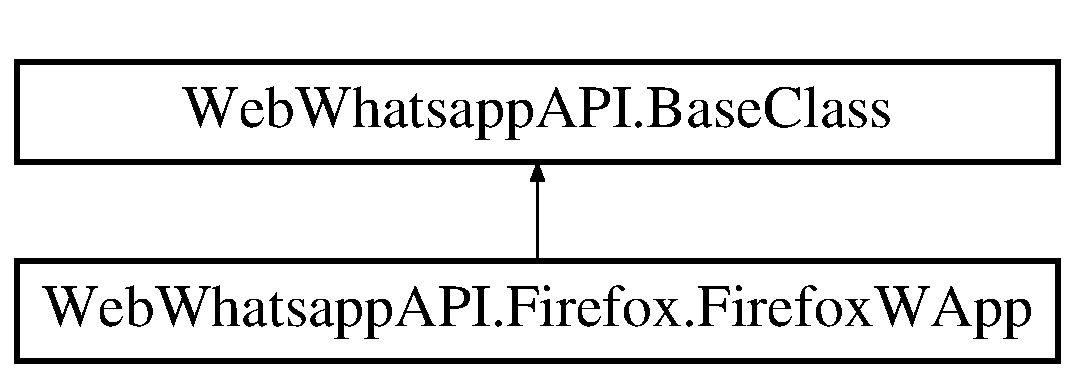
\includegraphics[height=2.000000cm]{class_web_whatsapp_a_p_i_1_1_firefox_1_1_firefox_w_app}
\end{center}
\end{figure}
\subsection*{Public Member Functions}
\begin{DoxyCompactItemize}
\item 
\hyperlink{class_web_whatsapp_a_p_i_1_1_firefox_1_1_firefox_w_app_a0c7a2248a6cf1699443a3ec99a17ba6d}{Firefox\+W\+App} ()
\begin{DoxyCompactList}\small\item\em Initialize \hyperlink{namespace_web_whatsapp_a_p_i_1_1_firefox}{Firefox} Driver \end{DoxyCompactList}\item 
override void \hyperlink{class_web_whatsapp_a_p_i_1_1_firefox_1_1_firefox_w_app_a80f406639e59bc4152b8f255962607f2}{Start\+Driver} ()
\begin{DoxyCompactList}\small\item\em Start the selenium engine and finalize the initialisation \end{DoxyCompactList}\end{DoxyCompactItemize}
\subsection*{Additional Inherited Members}


\subsection{Constructor \& Destructor Documentation}
\mbox{\Hypertarget{class_web_whatsapp_a_p_i_1_1_firefox_1_1_firefox_w_app_a0c7a2248a6cf1699443a3ec99a17ba6d}\label{class_web_whatsapp_a_p_i_1_1_firefox_1_1_firefox_w_app_a0c7a2248a6cf1699443a3ec99a17ba6d}} 
\index{Web\+Whatsapp\+A\+P\+I\+::\+Firefox\+::\+Firefox\+W\+App@{Web\+Whatsapp\+A\+P\+I\+::\+Firefox\+::\+Firefox\+W\+App}!Firefox\+W\+App@{Firefox\+W\+App}}
\index{Firefox\+W\+App@{Firefox\+W\+App}!Web\+Whatsapp\+A\+P\+I\+::\+Firefox\+::\+Firefox\+W\+App@{Web\+Whatsapp\+A\+P\+I\+::\+Firefox\+::\+Firefox\+W\+App}}
\subsubsection{\texorpdfstring{Firefox\+W\+App()}{FirefoxWApp()}}
{\footnotesize\ttfamily Web\+Whatsapp\+A\+P\+I.\+Firefox.\+Firefox\+W\+App.\+Firefox\+W\+App (\begin{DoxyParamCaption}{ }\end{DoxyParamCaption})\hspace{0.3cm}{\ttfamily [inline]}}



Initialize \hyperlink{namespace_web_whatsapp_a_p_i_1_1_firefox}{Firefox} Driver 



\subsection{Member Function Documentation}
\mbox{\Hypertarget{class_web_whatsapp_a_p_i_1_1_firefox_1_1_firefox_w_app_a80f406639e59bc4152b8f255962607f2}\label{class_web_whatsapp_a_p_i_1_1_firefox_1_1_firefox_w_app_a80f406639e59bc4152b8f255962607f2}} 
\index{Web\+Whatsapp\+A\+P\+I\+::\+Firefox\+::\+Firefox\+W\+App@{Web\+Whatsapp\+A\+P\+I\+::\+Firefox\+::\+Firefox\+W\+App}!Start\+Driver@{Start\+Driver}}
\index{Start\+Driver@{Start\+Driver}!Web\+Whatsapp\+A\+P\+I\+::\+Firefox\+::\+Firefox\+W\+App@{Web\+Whatsapp\+A\+P\+I\+::\+Firefox\+::\+Firefox\+W\+App}}
\subsubsection{\texorpdfstring{Start\+Driver()}{StartDriver()}}
{\footnotesize\ttfamily override void Web\+Whatsapp\+A\+P\+I.\+Firefox.\+Firefox\+W\+App.\+Start\+Driver (\begin{DoxyParamCaption}{ }\end{DoxyParamCaption})\hspace{0.3cm}{\ttfamily [inline]}, {\ttfamily [virtual]}}



Start the selenium engine and finalize the initialisation 



Reimplemented from \hyperlink{class_web_whatsapp_a_p_i_1_1_base_class_a8108d46b4176fc74fb49626e8122df88}{Web\+Whatsapp\+A\+P\+I.\+Base\+Class}.



The documentation for this class was generated from the following file\+:\begin{DoxyCompactItemize}
\item 
Web\+Whatsapp\+A\+P\+I/Firefox.\+cs\end{DoxyCompactItemize}

\hypertarget{class_web_whatsapp_a_p_i_1_1_base_class_1_1_msg_args}{}\section{Web\+Whatsapp\+A\+P\+I.\+Base\+Class.\+Msg\+Args Class Reference}
\label{class_web_whatsapp_a_p_i_1_1_base_class_1_1_msg_args}\index{Web\+Whatsapp\+A\+P\+I.\+Base\+Class.\+Msg\+Args@{Web\+Whatsapp\+A\+P\+I.\+Base\+Class.\+Msg\+Args}}


Arguments used by Msg event  


Inheritance diagram for Web\+Whatsapp\+A\+P\+I.\+Base\+Class.\+Msg\+Args\+:\begin{figure}[H]
\begin{center}
\leavevmode
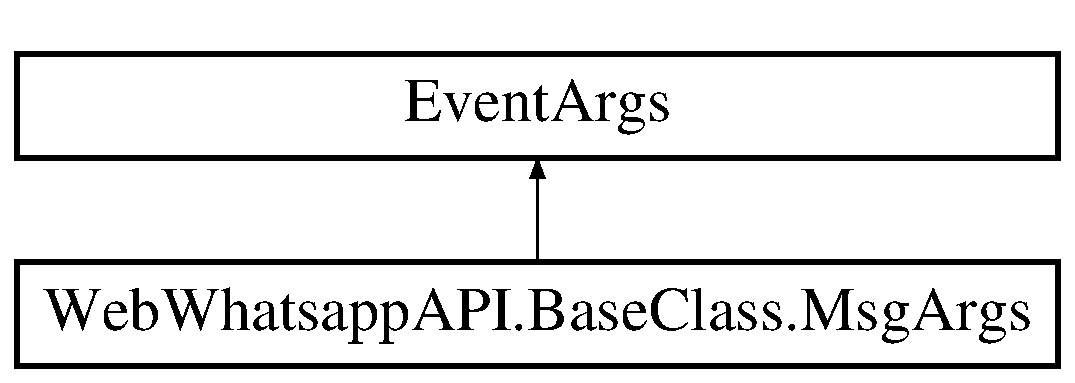
\includegraphics[height=2.000000cm]{class_web_whatsapp_a_p_i_1_1_base_class_1_1_msg_args}
\end{center}
\end{figure}
\subsection*{Public Member Functions}
\begin{DoxyCompactItemize}
\item 
\mbox{\Hypertarget{class_web_whatsapp_a_p_i_1_1_base_class_1_1_msg_args_aa15211e46707530747a91bb640791c3f}\label{class_web_whatsapp_a_p_i_1_1_base_class_1_1_msg_args_aa15211e46707530747a91bb640791c3f}} 
{\bfseries Msg\+Args} (string Message, string sender)
\end{DoxyCompactItemize}
\subsection*{Properties}
\begin{DoxyCompactItemize}
\item 
\mbox{\Hypertarget{class_web_whatsapp_a_p_i_1_1_base_class_1_1_msg_args_ad8b630e6df6ba85242a2f91316c71737}\label{class_web_whatsapp_a_p_i_1_1_base_class_1_1_msg_args_ad8b630e6df6ba85242a2f91316c71737}} 
string {\bfseries Msg}\hspace{0.3cm}{\ttfamily  \mbox{[}get\mbox{]}}
\item 
\mbox{\Hypertarget{class_web_whatsapp_a_p_i_1_1_base_class_1_1_msg_args_a9086dcdc39b06fde7c1b4b3dda710cfd}\label{class_web_whatsapp_a_p_i_1_1_base_class_1_1_msg_args_a9086dcdc39b06fde7c1b4b3dda710cfd}} 
string {\bfseries Sender}\hspace{0.3cm}{\ttfamily  \mbox{[}get\mbox{]}}
\item 
\mbox{\Hypertarget{class_web_whatsapp_a_p_i_1_1_base_class_1_1_msg_args_a3472dea941c91796a7ddce1ac3f73864}\label{class_web_whatsapp_a_p_i_1_1_base_class_1_1_msg_args_a3472dea941c91796a7ddce1ac3f73864}} 
Date\+Time {\bfseries Time\+Stamp}\hspace{0.3cm}{\ttfamily  \mbox{[}get\mbox{]}}
\end{DoxyCompactItemize}


\subsection{Detailed Description}
Arguments used by Msg event 



The documentation for this class was generated from the following file\+:\begin{DoxyCompactItemize}
\item 
Web\+Whatsapp\+A\+P\+I/Base\+Class.\+cs\end{DoxyCompactItemize}

\hypertarget{class_firefox_example_1_1_program}{}\section{Firefox\+Example.\+Program Class Reference}
\label{class_firefox_example_1_1_program}\index{Firefox\+Example.\+Program@{Firefox\+Example.\+Program}}


The documentation for this class was generated from the following file\+:\begin{DoxyCompactItemize}
\item 
Firefox\+Example/Program.\+cs\end{DoxyCompactItemize}

%--- End generated contents ---

% Index
\backmatter
\newpage
\phantomsection
\clearemptydoublepage
\addcontentsline{toc}{chapter}{Index}
\printindex

\end{document}
